\chapter{Introduction to Relational Databases in SQL}
\section{Uniquely identify records with key constraints}
\subsection{Keys and superkeys}

What is a key?
\begin{itemize}
    \item Attributes(s) that identify a record Uniquely.
    \item As long as attributes can be removed: \textbf{superkeys}.
    \item If no more attributes can be removed: minimal superkey or \textbf{key}.
\end{itemize}

\vspace{0.5em}
\begin{table}[ht]
    \centering
    \caption{Car database}
    \label{tab:carDB}
    \begin{tabular}{lllll}
\textbf{license\_no} & \textbf{serial\_no} & \textbf{make} & \textbf{model} & \textbf{year} \\
Texas ABC-739       & A69352              & Ford          & Mustang        & 2             \\
Florida TVP-347     & B43696              & Oldsmobile    & Cutlass        & 5             \\
New York MP0-22     & X83554              & Oldsmobile    & Delta          & 1             \\
California 432-TFY  & C43742              & Mercedes      & 190-D          & 99            \\
California RSK-629  & Y82935              & Toyota        & Camry          & 4             \\
Texas RSK-629       & U028365             & Jaguar        & XJS            & 4             \\
\end{tabular}
\end{table}

\emph{Note: Table adapted from Elmasri, Navathe (2011): Fundamentals of Database Systems, 6th Ed., Pearson}

SK1 = \{license\_no, serial\_no, make, model, year\} \\
SK2 = \{license\_no, serial\_no, make, model\} \\
SK3 = \{make, model, year\}, 
SK4 = \{license\_no, serial\_no\}, 
SKi, ..., SKn

A lot of possible superkeys with different combinations. But only four possible \textbf{keys}

K1 = \{license\_no\}; 
K2 = \{serial\_no\}; 
K3 = \{model\}; 
K4 = \{make, year\}

Here K1 to 3 only consist of one attribute. Removing either "make" or "year" from K4 would result in duplicates. Only one candidate key can be the chosen key.

A simple way of finding out whether a certain column(or combination) contains only unique values, wrap everything within the COUNT() function.

\inputminted[
    firstline=1,
    lastline=7,
    highlightlines={4-5},
]{SQL}{SQL/keys_and_superkeys.sql}

\section{Primary keys}
\begin{itemize}
    \item One primary key per database table, chosen from candidate keys
    \item Uniquely identifies records, e.g. for referencing in other tables
    \item Unique and not-null constraint both apply
    \item Should be built from as few column as possible
    \item Primary keys are time-invariant: choose columns wisely
\end{itemize}

\subsection{Specifying primary keys}

\inputminted[
    firstline=10,
    lastline=28,
    highlightlines={11,17,27}
]{SQL}{SQL/keys_and_superkeys.sql}

\emph{Note: Taken from PostgreSQL documentation.}

\subsection{Adding primary key to existing table}

\inputminted[
    firstline=30,
    lastline=31
]{SQL}{SQL/keys_and_superkeys.sql}

\section{Surrogate keys}
It is an artificial primary key that exist for the sole purpose of being a primary key.
Assume that a table consist of only make, model and year column from that table \ref{tab:carDB}

\subsection{Adding a surrogate key with serial data type}
Serial data type allow auto increment, and assign automatically when data is input.
\inputminted[
    firstline=33,
    lastline=34,
    highlightlines=34
]{SQL}{SQL/keys_and_superkeys.sql}

\subsection{Another type of surrogate key}
Combine two column to form a new ones for uniquely identifying
\inputminted[
    firstline=36,
    lastline=43,
    highlightlines=43
]{SQL}{SQL/keys_and_superkeys.sql}

\section{Glue together tables with foreign keys}
\subsection{Model 1:N relationships with foreign keys}

\begin{figure}[htbp]
    \centering
    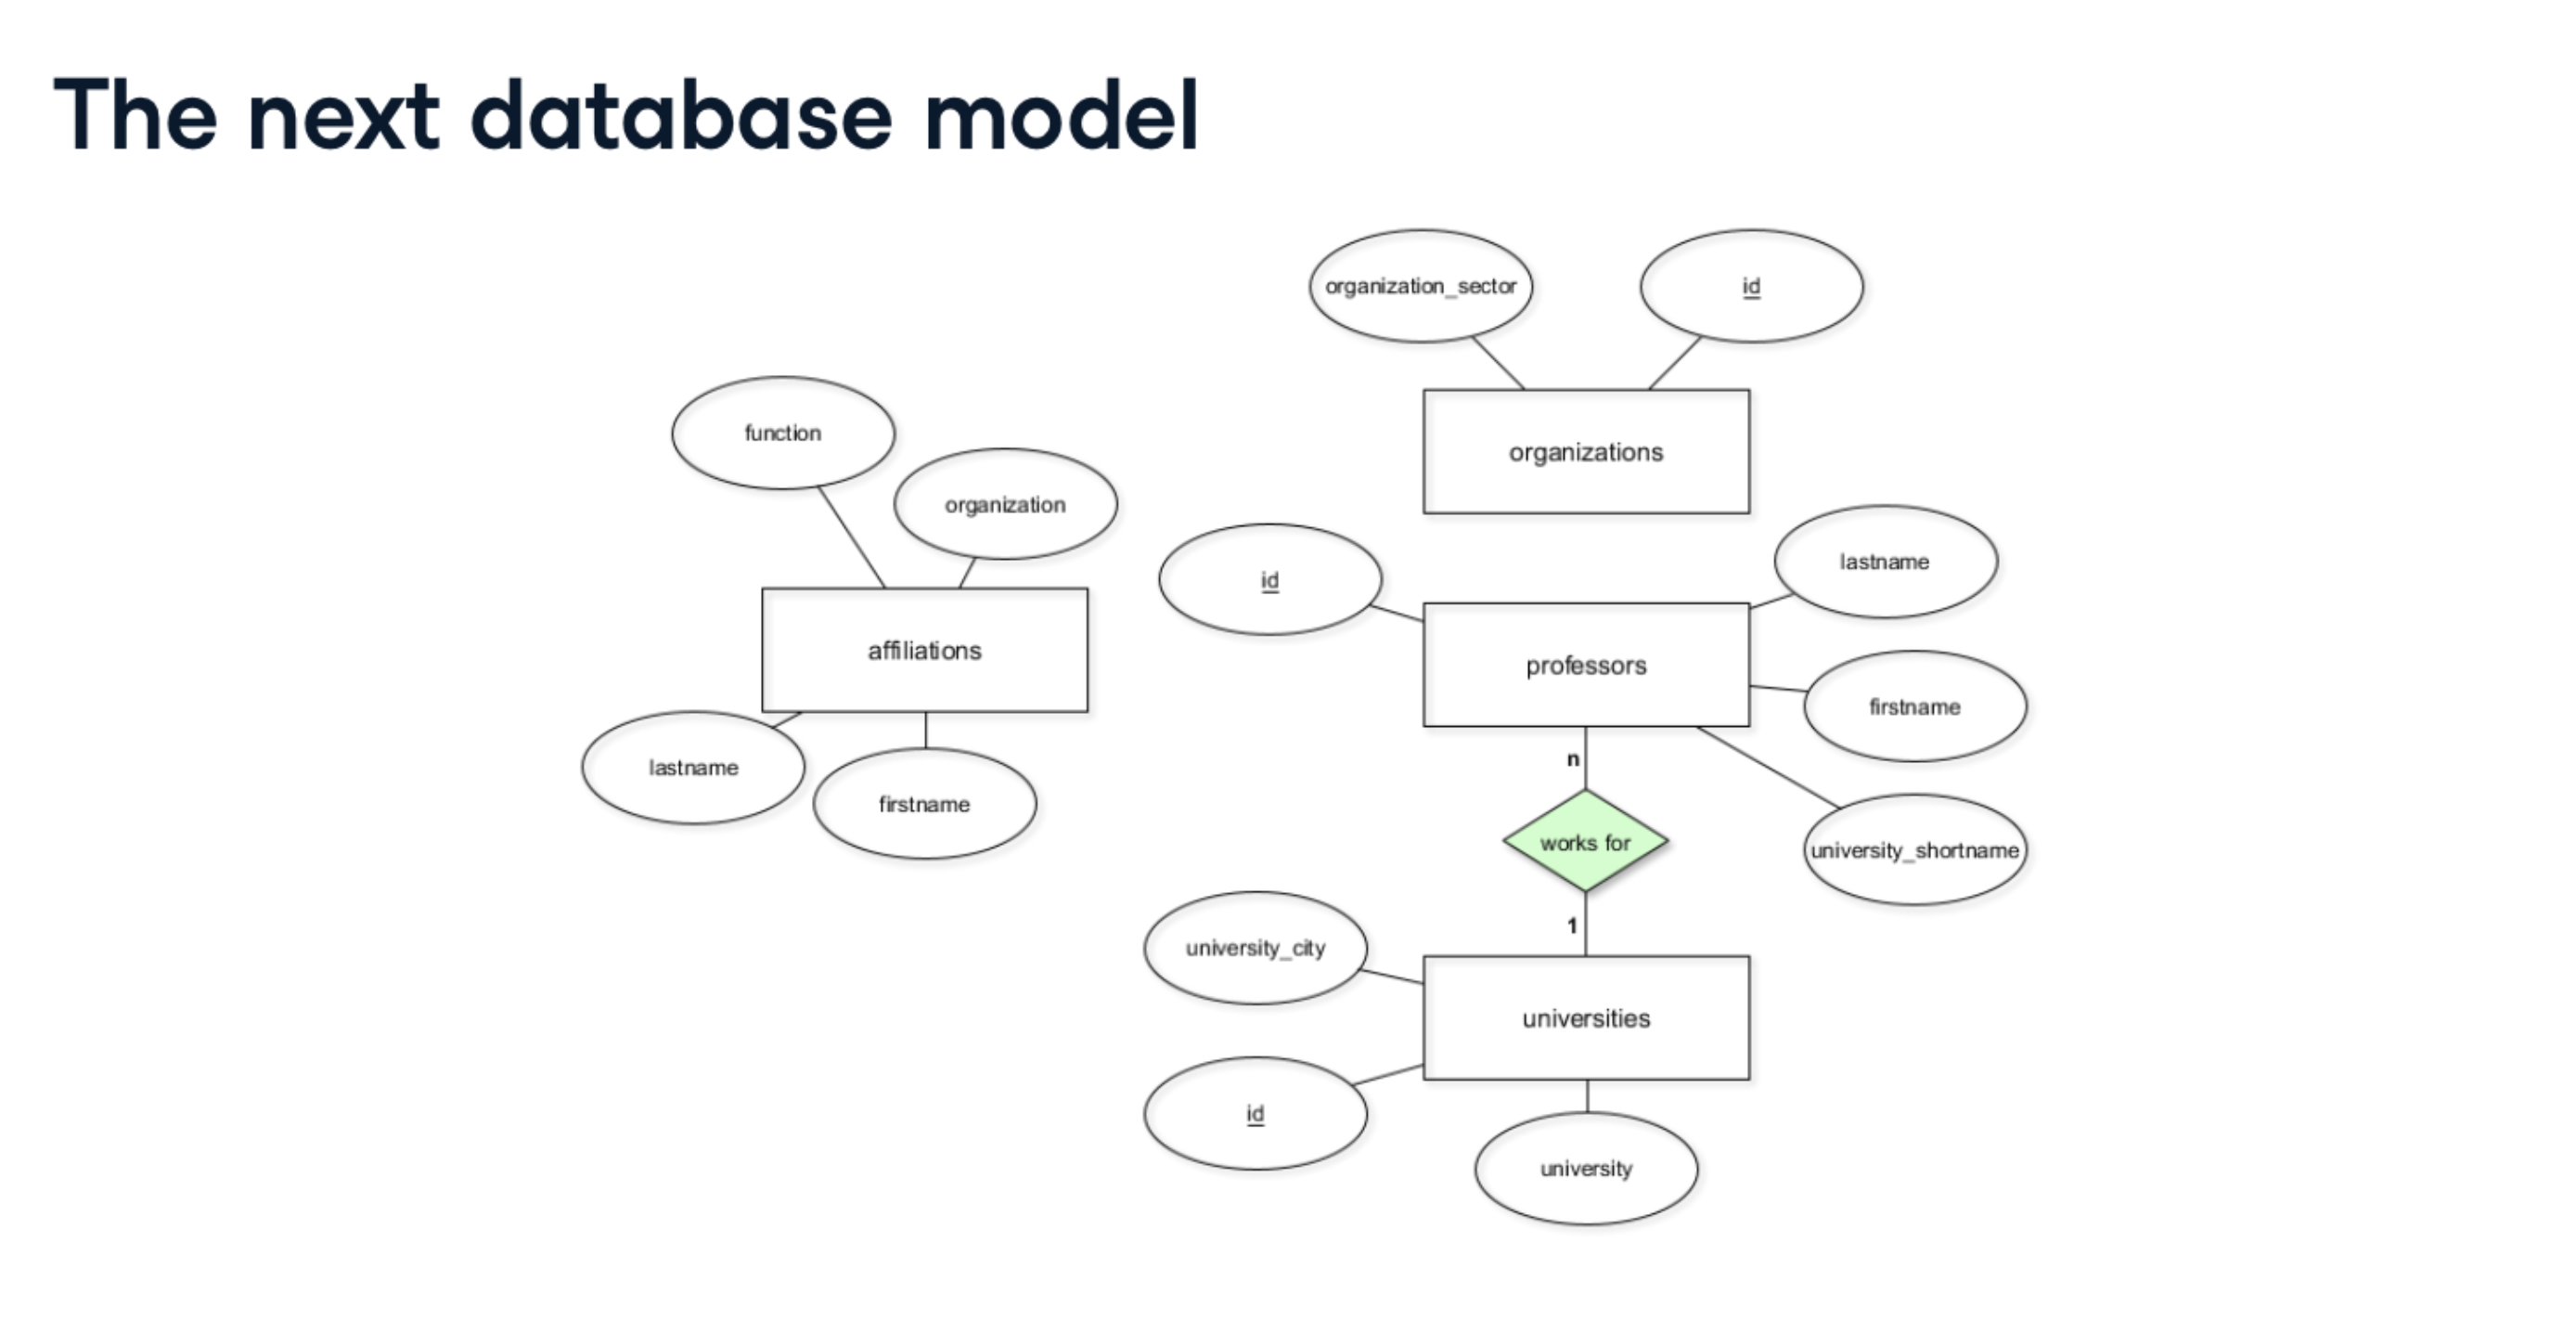
\includegraphics[width = 1.0\textwidth]{figures/relationship_er_diagram.png}
    \caption{Next ER diagram}
    \label{fig:ERDiagram}
\end{figure}
In the diagram \ref{fig:ERDiagram} Foreign key will add a one-to-many relationship where one university can have zero or more professors.

\subsubsection{Implementing relationship with foreign keys}
\begin{itemize}
    \item A foreign key (FK) points to the primary key (PK) of another table.
    \item Domain/data type of FK must be equal to domain of PK
    \item Each value of FK must exist in PK of another table (FK constraint or "referential integrity")
    \item FK are not actual keys as they can include null and duplicates values.
\end{itemize}

\subsubsection{Specifying foreign keys}

\inputminted[
    firstline=45,
    lastline=62,
    highlightlines=54
]{SQL}{SQL/keys_and_superkeys.sql}

\subsubsection{Specifying foreign keys to existing tables}
\inputminted[
    firstline=64,
    lastline=65,
    highlightlines=65
]{SQL}{SQL/keys_and_superkeys.sql}

\subsection{Model more complex relationships}
\begin{figure}[htbp]
    \centering
    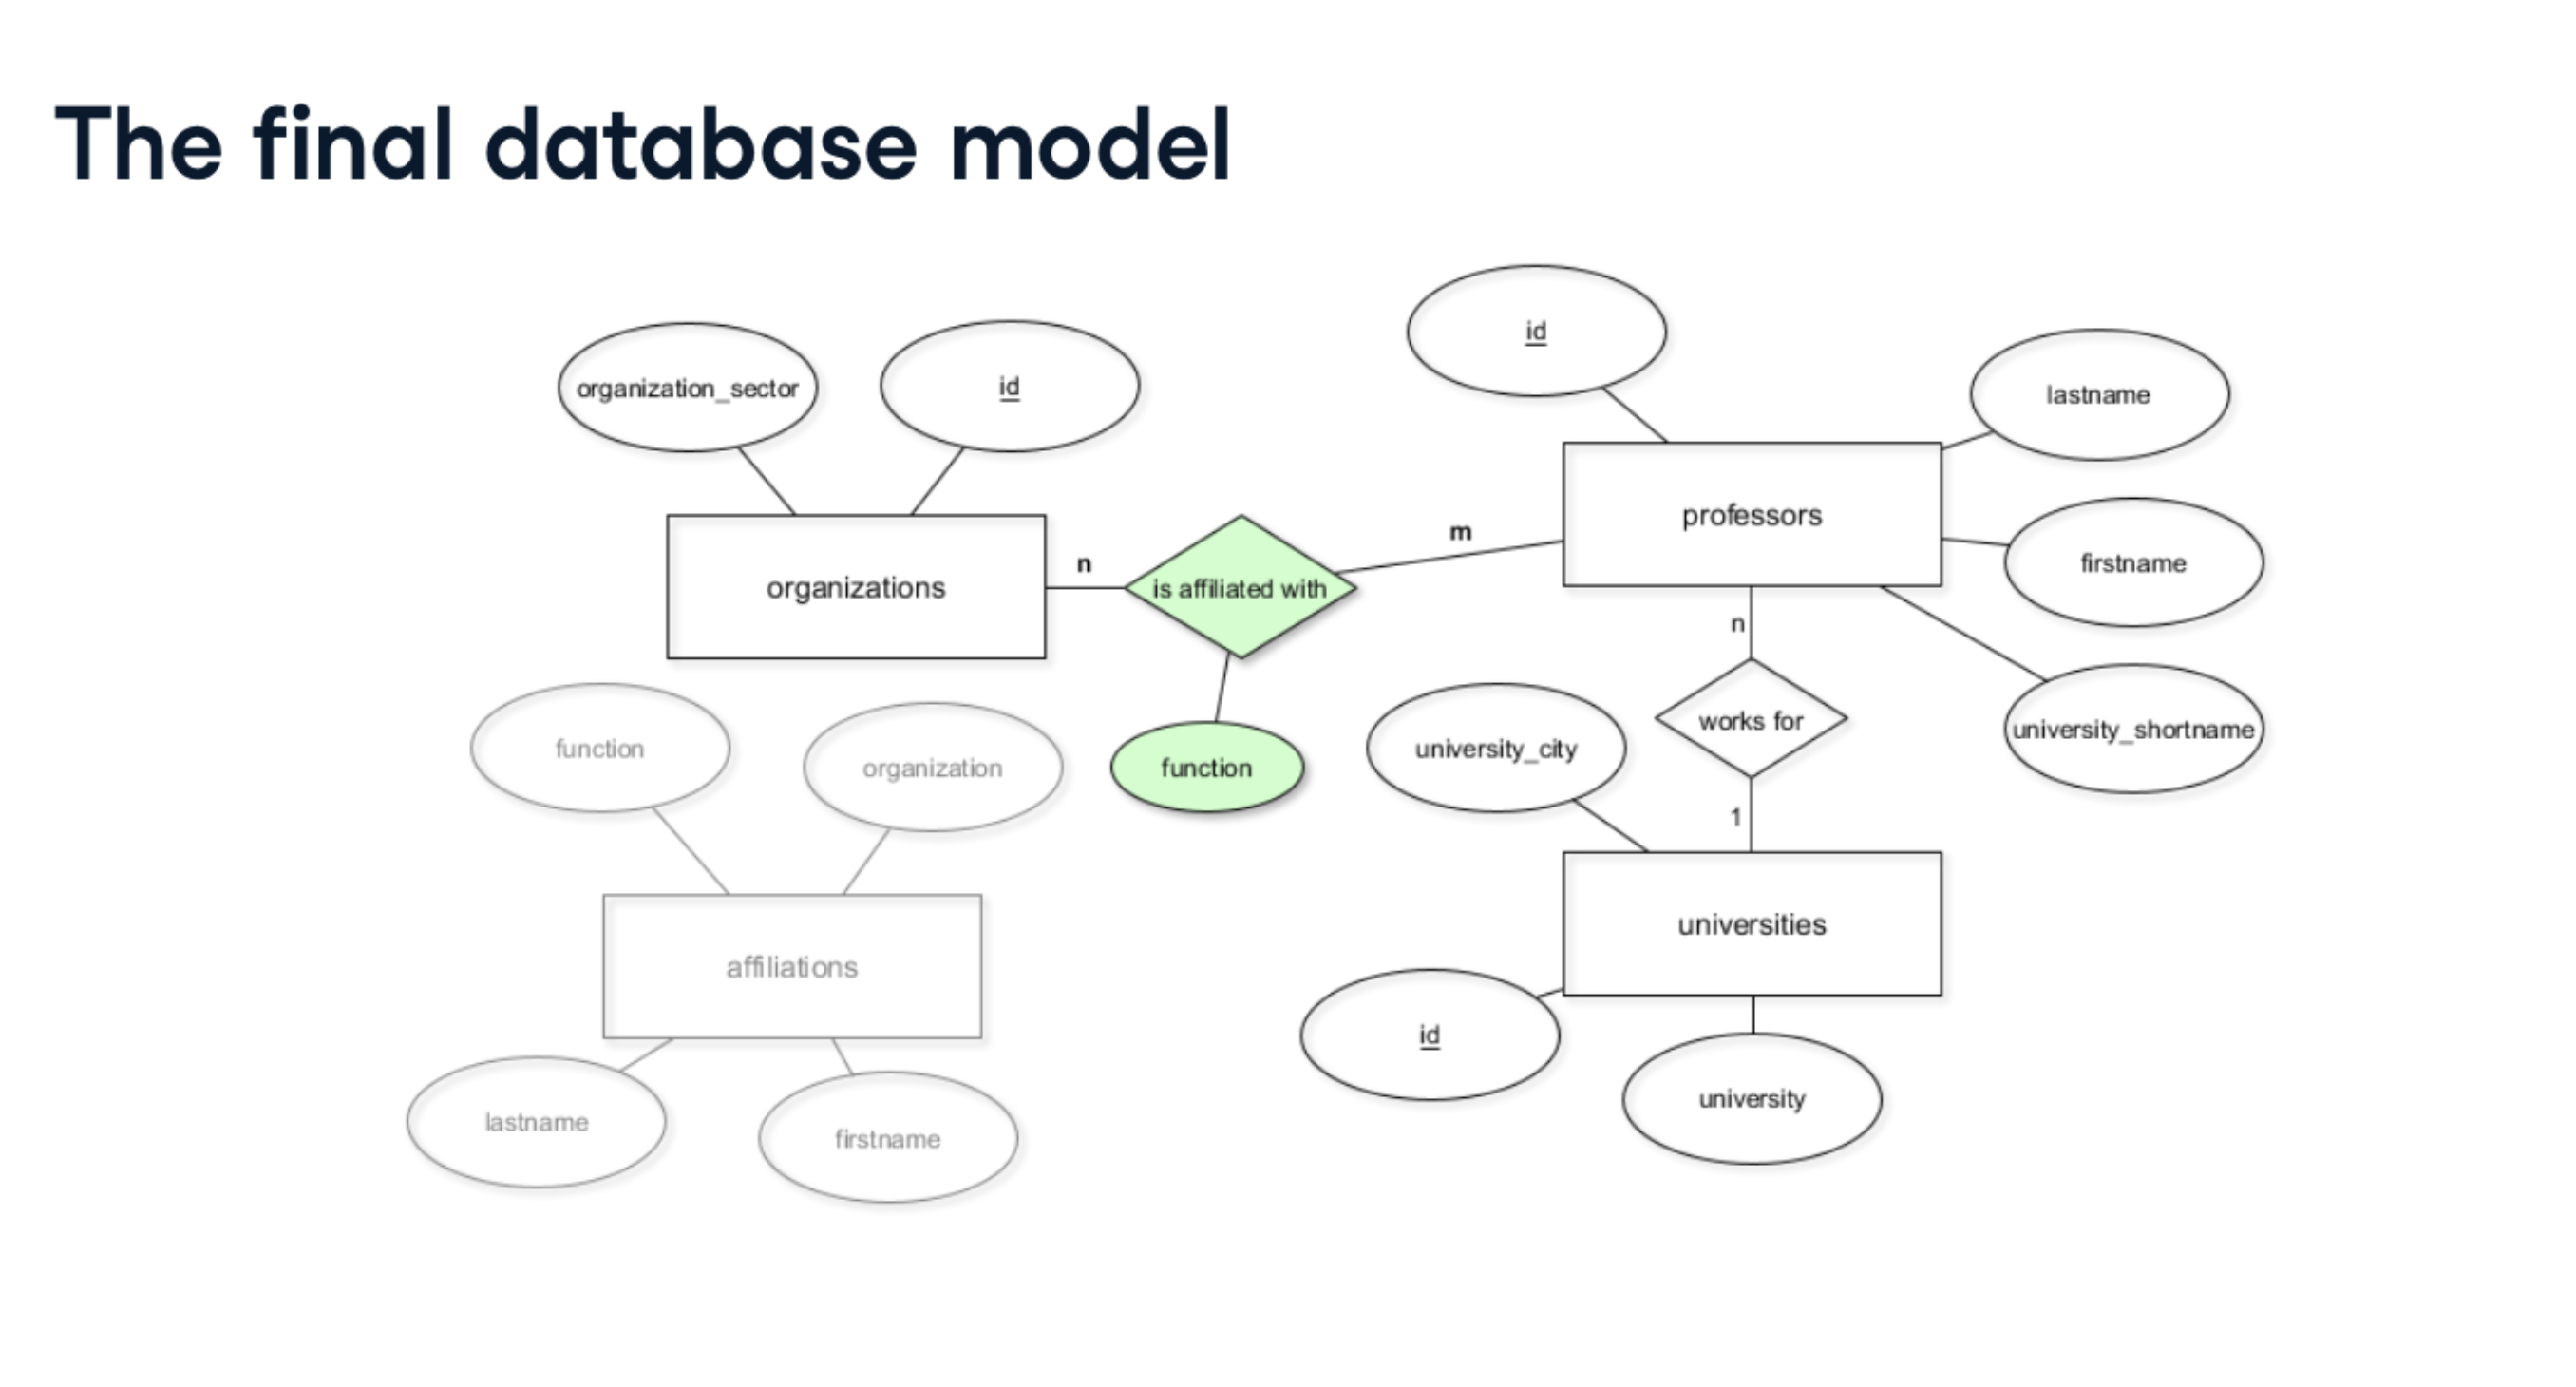
\includegraphics[width=1.0\textwidth]{figures/final_er_diagram.png}
    \caption{Final ER diagram}
    \label{fig:FinalERDiagram}
\end{figure}
In this diagram \ref{fig:FinalERDiagram} Foreign key enable many-to-many relationship
between organisation and professors, as professor can be affiliated with more than 1 
organisation and organisation itself can be associated with more than 1 professors.

\subsection{How to implement N:M-relationships}
\inputminted[
    firstline=67,
    lastline=71
]{SQL}{SQL/keys_and_superkeys.sql}
\begin{itemize}
    \item Create a table
    \item Add a foreign keys for every connected table
    \item Add additional attributes
    \item No primary key!
    \item Possible PK = \{professor\_id, organization\_id, function\}
\end{itemize}

\subsection{Referential integrity}
\begin{itemize}
    \item A record referencing another table must refer to an existing record in that Table
    \item Specified between two tables
    \item Enforced through foreign keys
\end{itemize}

\subsubsection{Referential integrity violations}
Referential integrity from table A to table B is violated...
\begin{itemize}
    \item ...if a record in table B that is referenced from a record in table A is deleted
    \item ...if a record in table A referencing a non-existing record from table B is inserted
    \item Foreign keys prevent violations!
\end{itemize}

\subsubsection{Dealing with violations}
\inputminted[
    firstline=73,
    lastline=85,
    highlightlines={77,84}
]{SQL}{SQL/keys_and_superkeys.sql}

ON DELETE
\begin{itemize}
    \item NO ACTION : Throw an error
    \item CASCADE : Delete all referencing records
    \item RESTRICT: Throw an error
    \item SET NULL : Set the referencing column to NULL
    \item SET DEFAULT : Set the referencing column to its default value, only work if default value is specified
\end{itemize}

\subsubsection{Drop existing constraint}
\inputminted[
    firstline=87,
    lastline=94
]{SQL}{SQL/keys_and_superkeys.sql}
